
%------------------------------------------------------------------------
% Anhänge
\appendix
\section{Appendix}
\subsection{Version Info}
\label{ref:versionInfo}
\begin{lstlisting}
1 VERSIONINFO
FILEVERSION 1,1,1,1
PRODUCTVERSION 1,1,1,1
FILEOS 0x4
FILETYPE 0x1
{
BLOCK "StringFileInfo"
{
	BLOCK "040904b0"
	{
		VALUE "CompanyName", "Valve"
		VALUE "FileDescription", "Half-Life Launcher"
		VALUE "FileVersion", "1, 1, 1, 1"
		VALUE "InternalName", "Half-Life Launcher"
		VALUE "LegalCopyright", "Copyright (c) 1996-2003"
		VALUE "LegalTrademarks", ""
		VALUE "OriginalFilename", "hl.exe"
		VALUE "ProductName", "Half-Life Launcher"
		VALUE "ProductVersion", "1, 1, 1, 1"
	}
}

BLOCK "VarFileInfo"
{
	VALUE "Translation", 0x0409 0x04B0
}
}
\end{lstlisting}

\newpage
\subsection{Abbildungen}

\begin{figure}[htbp]
	\centering
	
\includegraphics[scale=0.5]{bilder/EMail.png}
	\caption{Gefälschte UPS-Mail}
	\label{img:EMail}
\end{figure}

\begin{figure}[htbp]
	\centering
	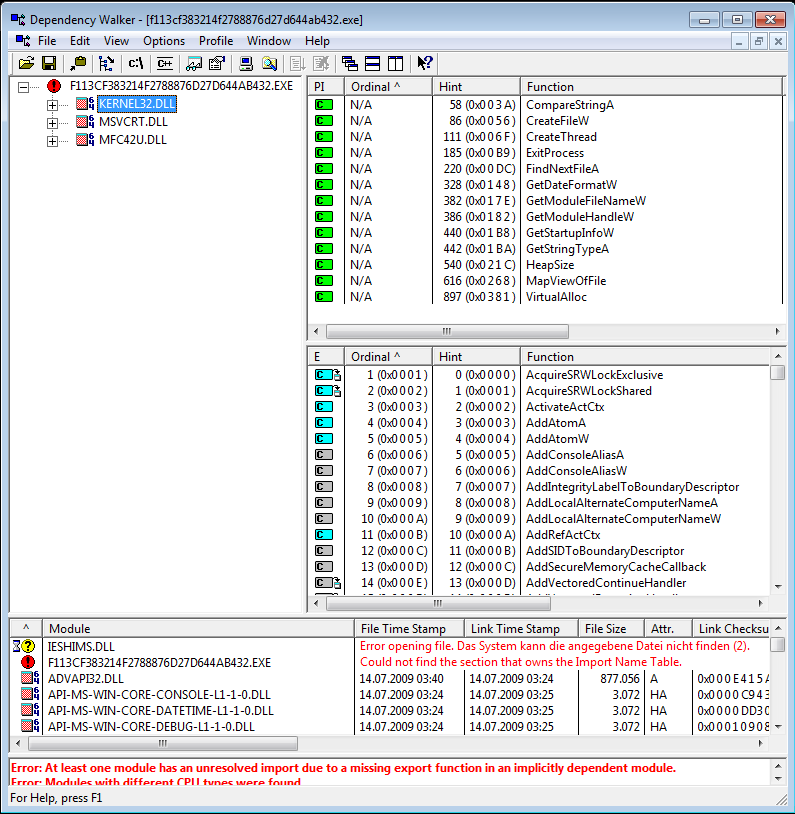
\includegraphics[scale=0.5]{bilder/statischeAnalyse/depWalker.png}
	\caption{Aufruf der Datei \textit{f113} mit dem Dependency Walker}
	\label{img:depWalkerf113}
\end{figure}

\begin{figure}[htbp]
	\centering
	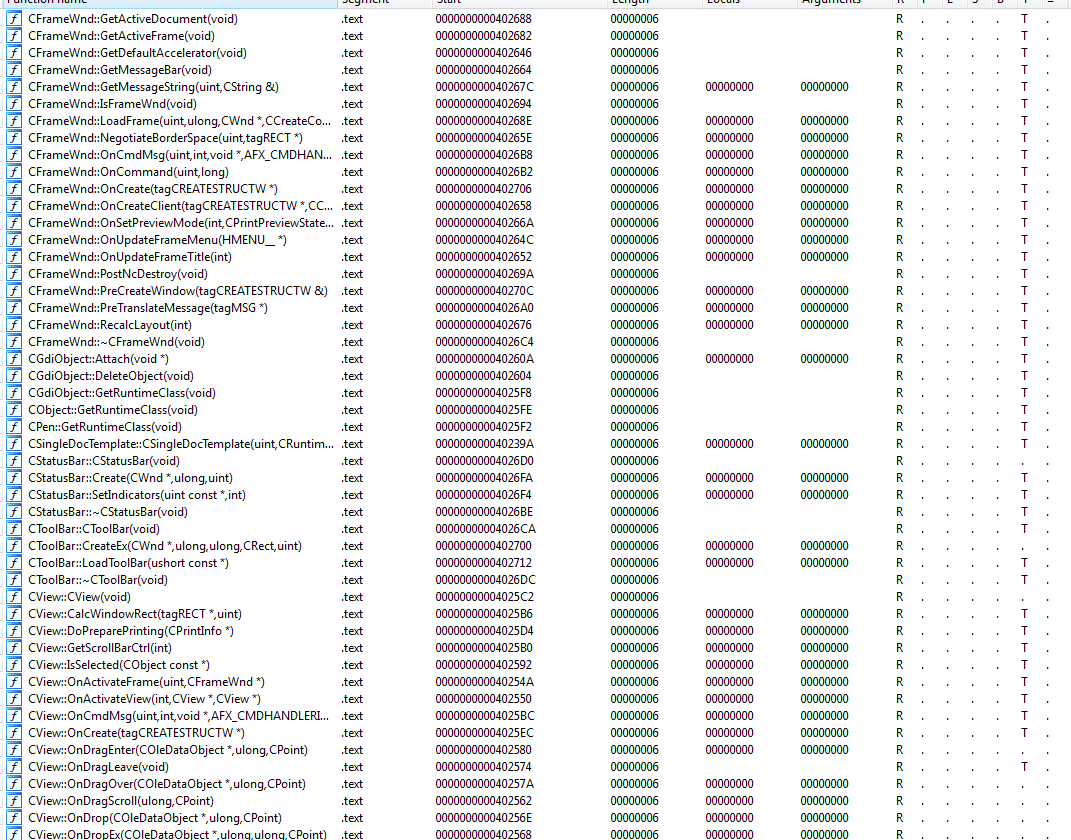
\includegraphics[width=\textwidth]{bilder/statischeAnalyse/IDAFunc.png}
	\caption{Funktionsaufrufe der Datei \textit{f113}, Ansicht in IDA}
	\label{img:IDAFuncf113}
\end{figure}

\begin{figure}[htbp]
	\centering
	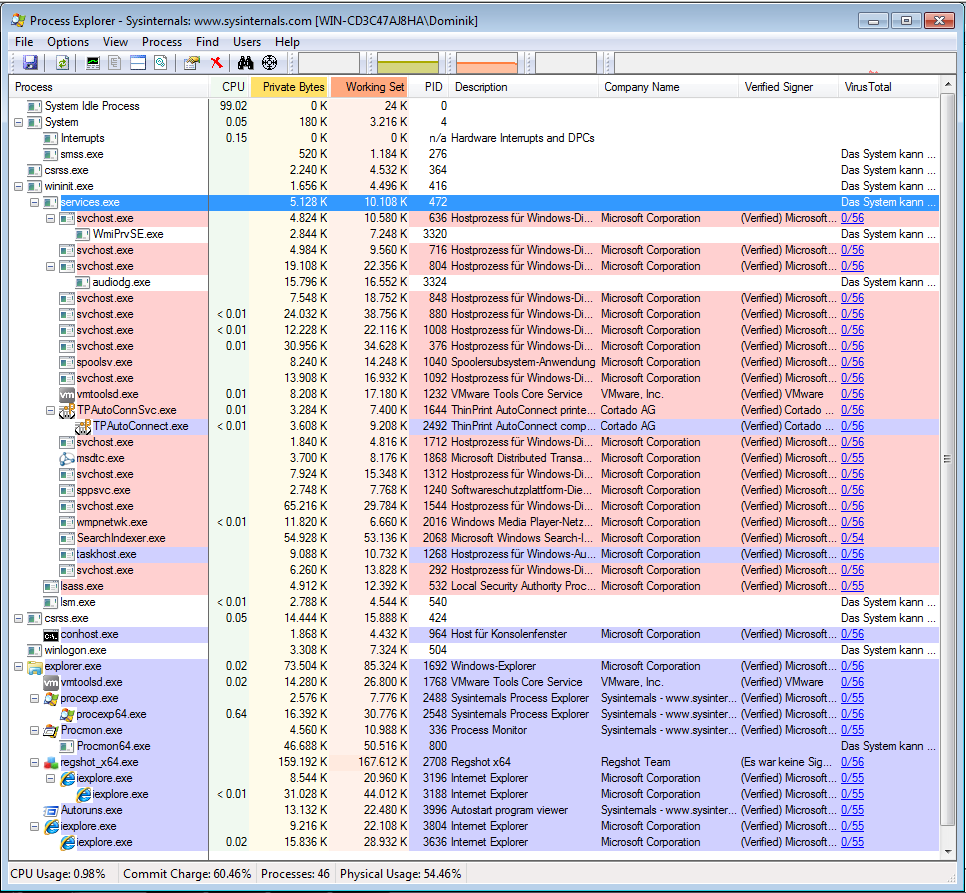
\includegraphics[width=\textwidth]{bilder/dynamischeAnalyse/ProcessExplorer.png}
	\caption{Process Explorer nach Ausführung von \textit{f113} mit Abgleich der Prozesse mit Virustotal}
	\label{img:ProcExpf113}
\end{figure}

\begin{figure}[htbp]
	\centering
	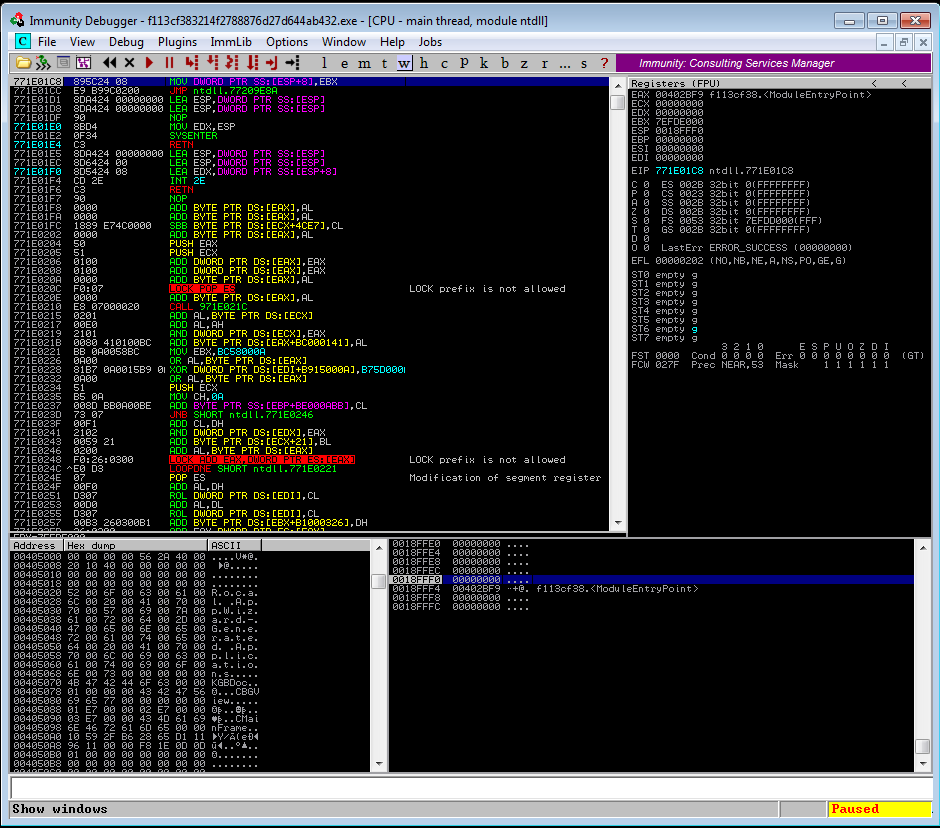
\includegraphics[width=\textwidth]{bilder/dynamischeAnalyse/ImmunityDebug.png}
	\caption{Hauptfenster des \textit{Immunity Debuggers} nach Ausführung von \textit{f113}}
	\label{img:ImmunityDebf113}
\end{figure}

\begin{figure}[htbp]
	\centering
	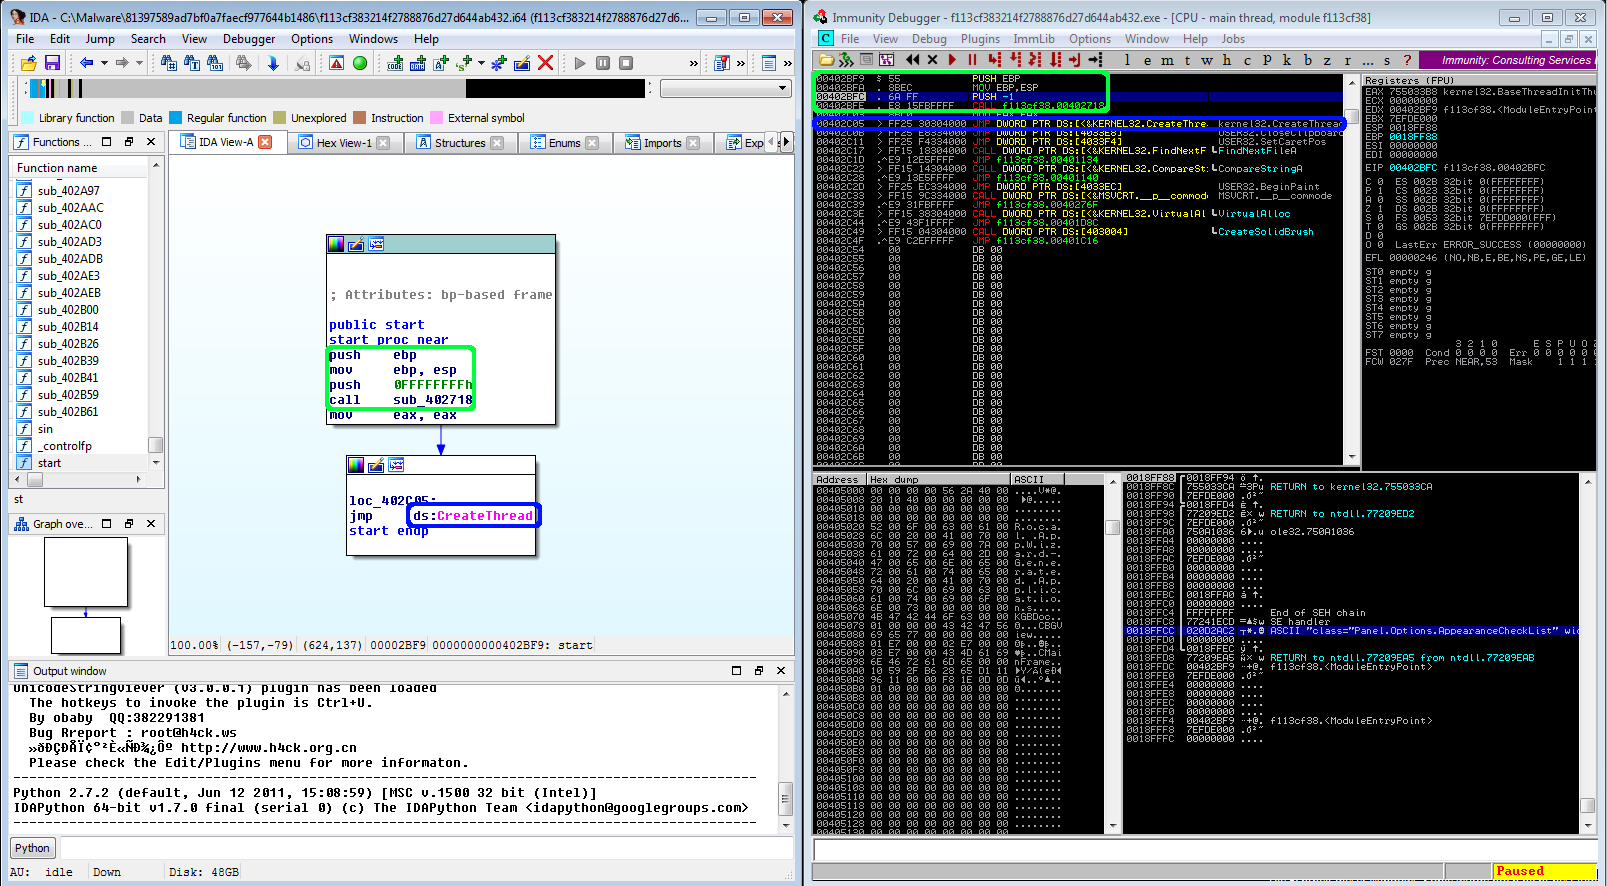
\includegraphics[angle=90, scale=.35]{bilder/dynamischeAnalyse/IDAtoImmunity.png}
	\caption{Zusammenhang von \textit{IDA} und \textit{Immunity Debuggers} bei \textit{f113}}
	\label{img:IDAtoImmunityf113}
\end{figure}

\begin{figure}[htbp]
	\centering
	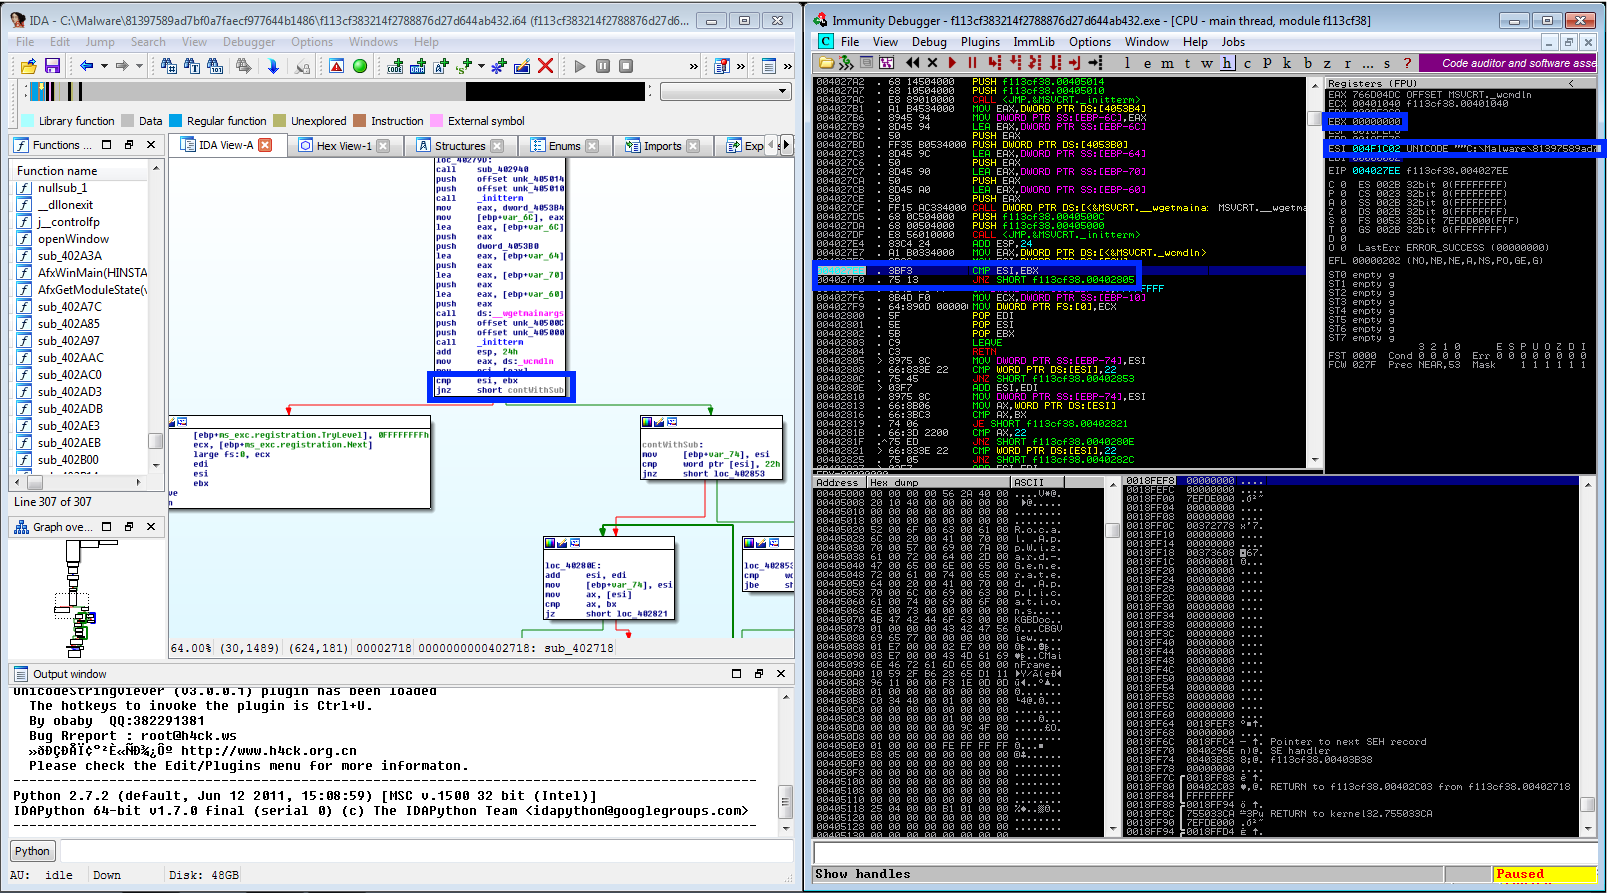
\includegraphics[angle=90, scale=.35]{bilder/dynamischeAnalyse/IDAtoImmunity2.png}
	\caption{Zusammenhang von \textit{IDA} und \textit{Immunity Debuggers} bei \textit{f113}}
	\label{img:IDAtoImmunity2f113}
\end{figure}